\section{Dataset} 
We collected the latest release (September, 2017) of Stack Exchange dataset. Stack Exchange is a network of community question answering websites where each site is based on a focused topic. Each user of Stack Exchange network participates in one or more of these sites based on their interest. The sites are diverse in terms of market characteristics, varying in theme (subject matter), size (number of users and volume of activity), and age (number of days in existence). 

There are 169 sites in our collected dataset. For the purpose of empirical analysis, we only consider the sites that have been active for at least 12 months beyond the ramp up period (site created, but few or no activity). There are 156 such sites. The age of these sites vary from 14 months to 111 months, number of user from 1072 to 547175, number of posts (questions and answers) from 1600 to 1985869. In addition, the sites have small overlaps in terms of user base, ranging from x\% to y\%. Therefore, we can reasonably consider the underlying markets as independent.

\iffalse
\begin{wrapfigure}{R}{0.2\textwidth}
\centering
\vspace{-\baselineskip}
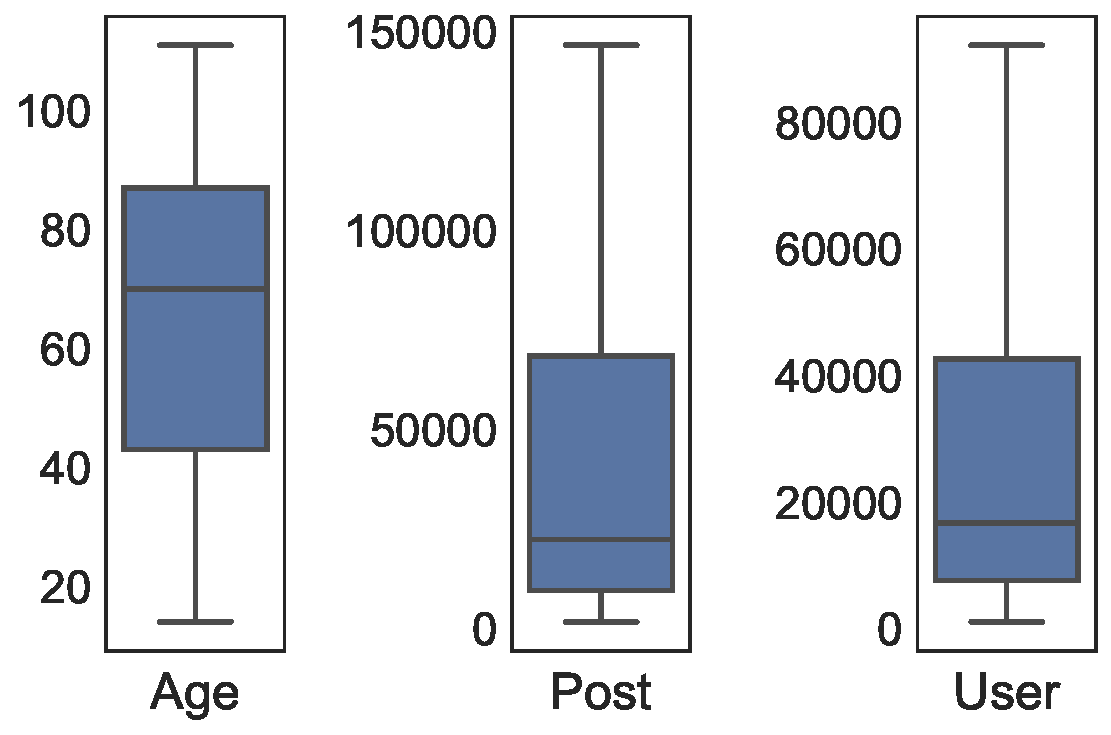
\includegraphics[width=0.2\textwidth]{Figures/Dataset_Statistics.pdf}
\caption{Site Statistics}
\vspace{-\baselineskip}
\end{wrapfigure}
\fi